\documentclass[12pt]{extarticle}
\usepackage[utf8]{inputenc}
\usepackage{graphicx}
\usepackage{float}

% Disable indentation
\setlength{\parindent}{0pt}

\title{Lab 1: Security Services, Algorithms with toolkit OpenSSL}
\author{Alexander Hoffmann}
\date{\today}

\begin{document}

\maketitle

\section{Hash function}
\textbf{a.} Using vim, we create a new file called \texttt{plain.txt} and type in "security lab". We can now print out the context of the file using the \texttt{cat} command.\\

\textbf{b.} We generate the hash values for the \texttt{plain.txt} file using \texttt{openssl}. The digest functions output the message digest of a supplied file or files in hexadecimal. The digest functions also generate and verify digital signatures using message digests.
\begin{verbatim}
openssl dgst -sha1 plain.txt >> hash.txt
\end{verbatim}
Now if we print the content of the file, we get the following output:
\begin{verbatim}
SHA1(plain.txt)= 8d678009606a414a6d163a1d96d832fddde1d3e4
\end{verbatim}

\textbf{c.} Now that we modified the content of the file, we generate another hash called \texttt{hash2.txt} using the same command as in question a.
\begin{verbatim}
openssl dgst -sha1 plain.txt >> hash2.txt
\end{verbatim}

\textbf{d.} We use \texttt{cat} to display the content of the new file. This time, we get another result.
\begin{verbatim}
SHA1(plain.txt)= 87a7acddb0d51bf22ed471c32215b1990f95aacb
\end{verbatim}
Hence, for every input, the hash function gives a different output. Note that for the same input, the SHA1 algorithm will give the same output.

\section{Symmetric Encryption}
Enc is used for various block and stream ciphers using keys based on passwords or explicitly provided. It can also be used for Base64 encoding or decoding.\\

Here are the arguments used:\\
\textbf{-cipher} - name of the cipher used, here des-cbc encryption method.\\
\textbf{-base64} - encode in a base64 format once it has been ecrypted.\\
\textbf{-k password} - Specify a password or a file containing the password which is used for key derivation.\\
\textbf{-in filename} - This specifies the input file.\\
\textbf{-out filename} - This specifies the output file. It will be created or overwritten if it already exists.\\

\textbf{a.} To encode a file \texttt{plain.txt} using password \texttt{ece}, we use the following command:
\begin{verbatim}
openssl enc -des-cbc -base64 -pbkdf2 -k ece -in plain.txt -out cipher.txt
\end{verbatim}

\textbf{b.} Now we want to decode the file we previously encoded. To do this, use:
\begin{verbatim}
openssl enc -des-cbc -base64 -pbkdf2 -k ece -in cipher.txt -d -out newplain.txt
\end{verbatim}
Finally, verify that both file are the same using \texttt{diff plain.txt newplain.txt} which yields no result at all, meaning both files are identical hence the encoding and decoding worked perfectly.\\\\
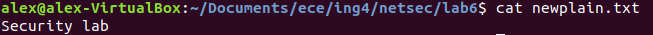
\includegraphics[scale=0.6]{resources/1.png}

\section{Asymmetric Encryption}
\textbf{a.} The genrsa command generates an RSA private key. To generate key with size 2048, we use:
\begin{verbatim}
openssl genrsa -out privMyName.key 2048
\end{verbatim}

\textbf{b.} The rsa command processes RSA keys. They can be converted between various forms and their components printed out. To generate a public key from a private key, use:
\begin{verbatim}
openssl rsa -in privMyName.key -out pubMyName.key -pubout 
\end{verbatim}

\textbf{c.} The rsautl command can be used to sign, verify, encrypt and decrypt data using the RSA algorithm. To encrypt our \texttt{plain.txt} file, we use:
\begin{verbatim}
openssl rsautl -encrypt -pubin -inkey pubMyName.key -in plain.txt -out cipherrsa.txt
\end{verbatim}
Now let's decrypt the file we just created using our private key.
\begin{verbatim}
openssl rsautl -decrypt -inkey privMyName.key -in cipherrsa.txt -out newplain2.txt
\end{verbatim}
If we use \texttt{diff} to print the differences between both files, we will see that they are the same. This means that our encryption has worked correctly.\\\\
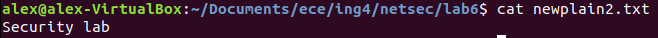
\includegraphics[scale=0.6]{resources/2.png}

\section{Asymmetric/Symmetric Encryption, Digital signature}
\textbf{a.} Alice wants to send a private message to Bob but she doesn't want anyone to be able to read the content of the message. She decides to find a way to send messages to Bob without anyone else being able to read them: symmetric-key encryption.\\
Alice and Bob agree on a key K in private. Now they can talk aloud, encoding messages with the key.\\
Alice and Bob can't communicate a key in advance in private. This is a job for public-key cryptography. Now Bob has two keys, one (P) published, one (K) kept secret. A message encrypted with the public key P can only be decrypted with the private key K.\\
Alice gets P from Bob, encrypts a message, and sends it to Bob. Bob uses K to decrypt the message.
A listener in the middle can easily get P, but cannot decrypt the message!\\
Alice and Bob agree on a key K in private. Now they can talk aloud, encoding messages with the key.\\

\textbf{b.} The rand command outputs n pseudo-random bytes after seeding the random number generator once. To generate a symmetric key, use:
\begin{verbatim}
openssl rand -out sym.key -hex 16
\end{verbatim}

\textbf{c.} Using \texttt{vim}, we create a new file called \texttt{plaintext.txt} containing the following sentence "My Security LAB: My Name is Alex".\\
Next, we generate two private RSA keys and export the public keys corresponding using the following commands:
\begin{verbatim}
openssl genrsa -out privA.key
openssl rsa -in privA.key -out pubA.key -pubout
\end{verbatim}
For key A and
\begin{verbatim}
openssl genrsa -out privB.key
openssl rsa -in privB.key -out pubB.key -pubout
\end{verbatim}
for key B.

\textbf{d.} Encrypt our plain text file using
\begin{verbatim}
openssl enc -aes-128-cbc -base64 -pbkdf2 -kfile sym.key -in plaintext.txt -out ciphertext.txt
\end{verbatim}

\textbf{e.} Encrypt the symmetric key using
\begin{verbatim}
openssl rsautl -encrypt -pubin -inkey pubB.key -in sym.key -out secret.key
\end{verbatim}

\textbf{f.} Generate the hash value of the key
\begin{verbatim}
openssl dgst -sha1 secret.key >> sym.sha1
\end{verbatim}

\textbf{g.} Sign the hashed value file
\begin{verbatim}
openssl rsautl -sign -inkey privA.key -in sym.sha1 -out sym.sig
\end{verbatim}

After all of this is set and done, we have all the necessary files to have a secret conversation between Alice and Bob. Here is what the folder looks like.\\\\
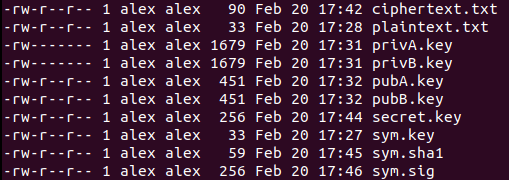
\includegraphics[scale=0.6]{resources/3.png}
A copy of the folder is attached as a zip.\\

\textbf{h.} Now it's time to decrypt the secret message we receibed from Alice. Here are the steps to recover the plain text file:
\begin{verbatim}
openssl rsautl -verify -pubin -inkey pubA.key -in sym.sig -out sym.sha1
openssl dgst -sha1 secret.key
openssl rsault -decrypt -inkey privB.key -in secret.key -out sym.key
openssl enc -aes-128-cbc -d -base64 -kfile sym.key -in ciphertext.txt -out plaintext.txt
\end{verbatim}
Here is the result on the other machine:\\\\
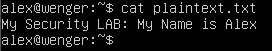
\includegraphics[scale=0.9]{resources/4.png}

\textbf{d.} Advantages\\
- encrypted data can be transferred on the link even if there is a possibility that the data will be intercepted\\
- only a user who possesses the secret key can decrypt a message\\
- the receiver can be sure of the identity of the sender because only both of them have the private key.

\end{document}
